\section{Arquitetura do Framework}
\label{sec:architecture}

Este capítulo apresenta a metodologia para avaliar como perturbações ambientais 
e climáticas reduzem a acessibilidade urbana e afetam diferentes grupos sociais. 
O método consiste em comparar quantitativamente dois cenários da rede de deslocamento: 
um com condições típicas e outro modificado por variáveis ambientais. Essa 
comparação permite isolar, quantificar e mapear as perdas de acesso às oportunidades 
na cidade.

\begin{figure}[H]
  \centering
  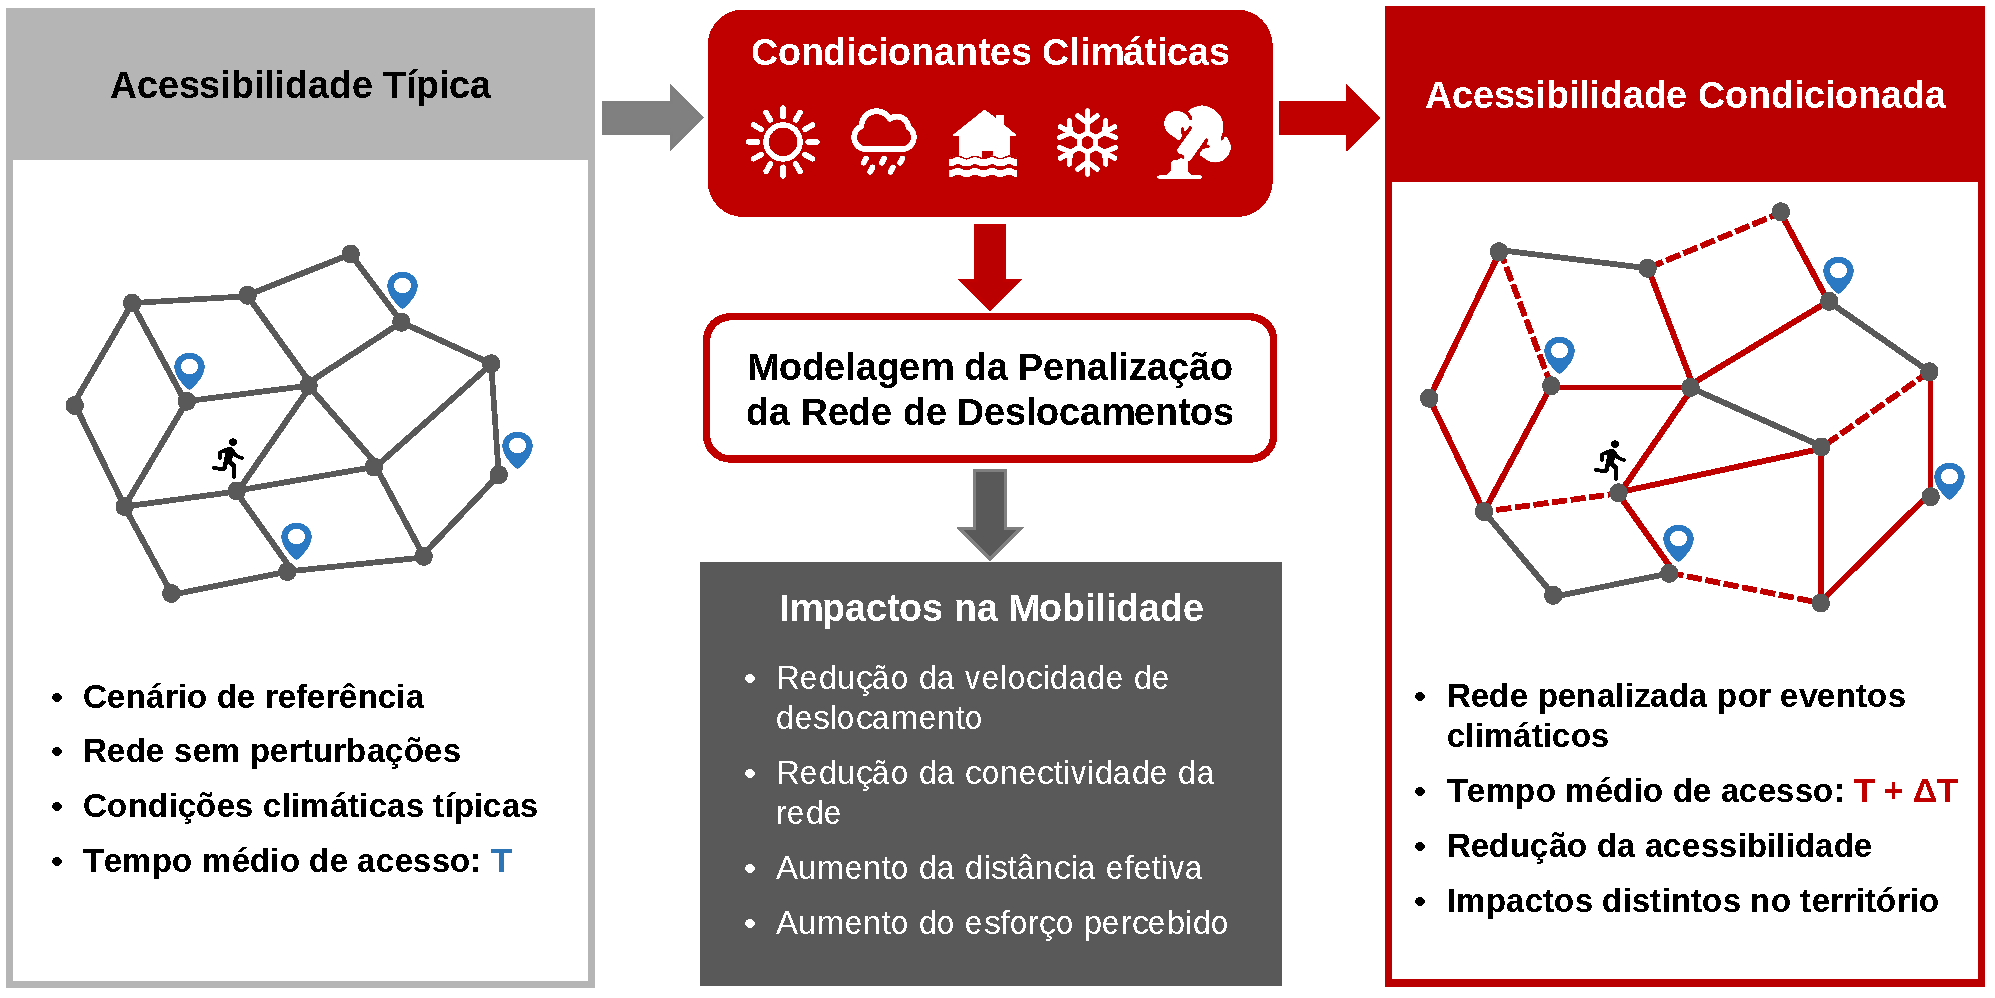
\includegraphics[width=1\textwidth]{figs/framework.pdf}
  \caption{Fluxo de modelagem dos cenários de acessibilidade. À esquerda, a rede no cenário típico, com seus custos originais de deslocamento. Ao centro, o mecanismo de penalização, que utiliza dados ambientais para penalizar a infraestrutura de mobilidade. À direita, o cenário condicionado, no qual o aumento do comprimento das arestas representa visualmente o acréscimo no tempo ou custo de deslocamento provocado pela perturbação.}
  \label{fig:framework}
\end{figure}

\subsection{Modelagem Territorial}
\label{subsec:territorial_modelling}

A modelagem do território urbano consiste na coleta, pré-processamento e integração de cinco camadas de dados espaciais que servem de base para a análise da acessibilidade:

\paragraph{1. Malha de análise:} Uma grade espacial regular que define a unidade mínima de estudo. A resolução da malha é ajustada ao modo de transporte e ao contexto local. O centroide de cada célula funciona como a origem teórica dos deslocamentos, servindo de base para o cálculo e a agregação dos indicadores.

\paragraph{2. Pontos de Interesse (POIs):} Representam os destinos dos deslocamentos. São coordenadas que indicam a localização dos serviços cotidianos da população, organizados em categorias (como saúde, educação e transporte). A seleção depende da disponibilidade de bases de dados locais, sejam oficiais ou colaborativas (crowdsourced).

\paragraph{3. Rede viária:} A infraestrutura de mobilidade é estruturada como um grafo espacial. Os vértices representam os cruzamentos e as arestas representam os segmentos de via, cujo peso base inicial corresponde à distância percorrida. Para possibilitar o cálculo de rotas reais, o centroide de cada célula da malha de análise é vinculado ao vértice mais próximo da rede.

\paragraph{4. Condicionantes ambientais:} Camadas espaciais, que podem ser contínuas (como imagens \textit{raster}) ou discretas (polígonos vetoriais), mapeando os fenômenos climáticos ou ambientais avaliados. Esses dados são sobrepostos à rede viária para reajustar o custo de deslocamento das arestas afetadas no cenário perturbado.

\paragraph{5. Dados Demográficos e Socioeconômicos:} Informações que caracterizam a população residente, como densidade demográfica, renda e escolaridade, oriundas de censos oficiais. Como esses dados são disponibilizados em unidades administrativas irregulares (como setores censitários), aplica-se um procedimento de compatibilização espacial para transferir o perfil socioeconômico para as células da malha regular de análise.
